%************************************************
\chapter{Platform Specific Functionality}\label{ch:ui}
%************************************************

Thanks to the framework we chose to use, and the desire to present our application as natively as possible, there exists the need for some platform specific functionality. Most of this functionality has to do with the \ac{UI} and some third-party libraries.

This chapter will be divided in two parts, one for iOS and one for Android. In here we will also discuss all about the \texttt{callback} functions we mentioned earlier. 

\section{Android UI}

The main reason we chose \textit{Xamarin} as the framework for the development of our application is the fact that we can develop the \ac{UI} in a completely independent fashion.

On the Android side of things, this means using specially crafted \ac{XML} files for defining the look of the application. Under Xamarin Studio, we have two options for laying out the content of each view:  We can use the Android Layout Editor to drag and drop elements form a toolbox or we can  directly edit the \ac{XML} source code and change everything manually.

Since most of the application is composed of Lists and Grids, it is actually easier to manually edit the \ac{XML} source code, than to mess around with the visual editor.

\autoref{list:and_xml} and \autoref{fig:and_layout} show both sides of the same file, the source and how it looks inside the Android Layout Editor.

What each element inside the \ac{XML} file is, how they work and why they work that way is outside the scope of this work. If you need more information about the inner workings of the Android Operating System, please refer to more specific literature.


\lstset{language=XML}
\begin{lstlisting}[frame=lt,caption=Company.axml, label={list:and_xml}]
<?xml version="1.0" encoding="utf-8"?>
<LinearLayout xmlns:android="http://schemas.android.com/apk/res/android"
    android:orientation="vertical"
    android:layout_width="wrap_content"
    android:layout_height="wrap_content">
    <ImageView
        android:src="@android:drawable/ic_menu_gallery"
        android:layout_width="match_parent"
        android:layout_height="match_parent"
        android:padding="5dip"
        android:gravity="center"
        android:id="@+id/company_image" />
    <TextView
        android:id="@+id/Name"
        android:layout_width="match_parent"
        android:layout_height="wrap_content"
        android:ellipsize="end"
        android:singleLine="true"
        android:textAppearance="?android:attr/textAppearanceSmall"
        android:padding="5dip"
        android:gravity="center"
        android:text="Test" />
</LinearLayout>
\end{lstlisting}


\begin{figure}[H]
    \begin{center}
        {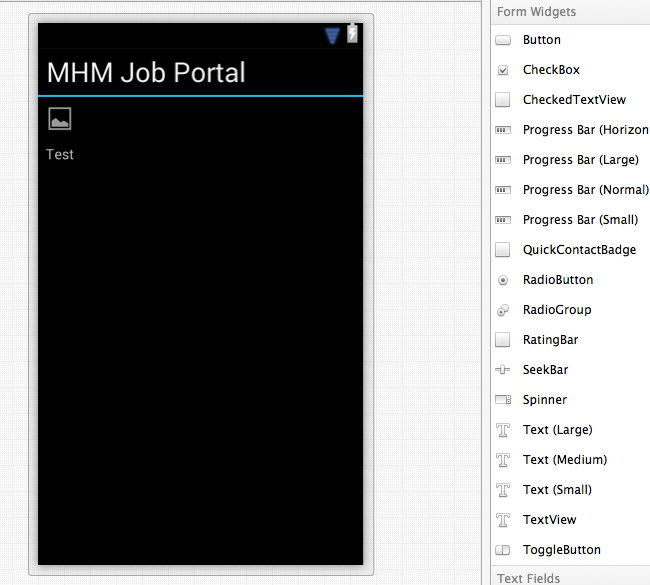
\includegraphics[width=0.75\linewidth]{gfx/and_view}}
        \caption[Android Layout Editor]{Android Layout Editor}\label{fig:and_layout}
    \end{center}
\end{figure}

\subsection{List Views, Items and Adapters}
Our Job Portal Aggregator consists of information that is easily packable inside a list, this is why the main view of the application consists of a list of the latest vacancies available.

In order to display this information we need to define a view group where the information will be placed and a view item that represents each element inside the list. All these is done inside the \ac{XML} layout files.

\begin{lstlisting}[frame=lt,caption=Publication.axml, label={list:pub_xml}]
<?xml version="1.0" encoding="utf-8"?>
<LinearLayout xmlns:android="http://schemas.android.com/apk/res/android"
    android:orientation="horizontal"
    android:layout_width="fill_parent"
    android:layout_height="fill_parent">
    <ImageView
        android:src="@android:drawable/ic_menu_gallery"
        android:layout_width="57.2dp"
        android:layout_height="63.0dp"
        android:id="@+id/company_image" />
    <LinearLayout
        android:orientation="vertical"
        android:layout_width="fill_parent"
        android:layout_height="fill_parent">
        <TextView
            android:id="@+id/Title"
            android:layout_width="match_parent"
            android:layout_height="wrap_content"
            android:ellipsize="end"
            android:singleLine="true"
            android:textAppearance="?android:attr/textAppearanceMedium"
            android:padding="5dip"
            android:text="Test" />
        <TextView
            android:id="@+id/Description"
            android:layout_width="match_parent"
            android:layout_height="wrap_content"
            android:padding="5dip"
            android:text="Test" />
    </LinearLayout>
</LinearLayout>
\end{lstlisting}

\autoref{list:pub_xml} describes a Publication element and defines how it will be shown inside the main list. It features the company logo (\texttt{<ImageView>}), the Publication's Title just to the right of the image and its Short Description just bellow the title.

But this is just for one item, we need to define the list that will hold a collection of Publications. In \autoref{list:pubList_xml} we can see that all that is needed is a \texttt{ListView} item. 

\begin{lstlisting}[frame=lt,caption=PublicationsList.axml, label={list:pubList_xml}]
<?xml version="1.0" encoding="utf-8"?>
<LinearLayout xmlns:android="http://schemas.android.com/apk/res/android"
    android:id="@+id/pub_list"
    android:orientation="vertical"
    android:layout_width="fill_parent"
    android:layout_height="fill_parent">
    <ListView
        android:id="@+id/Publications"
        android:layout_width="match_parent"
        android:layout_height="wrap_content" />
</LinearLayout>
\end{lstlisting}

Now that we have defined the list and the appearance of each item within it, we need to connect these elements with real data. That's where adapters come into play. 

\texttt{Adapters} are in charge of populating the list using a collection of items that gets passed via the constructor. They implement a \texttt{GetView} method that matches elements from the actual object to its visual representation inside the list and define some simple methods for member data accessibility.

\lstset{language=[Sharp]C}

\begin{lstlisting}[frame=lt,caption=PublicationsListAdapter.cs, label={list:pubList_cs}]
class PublicationsListAdapter : BaseAdapter<Publication> {
	readonly LayoutInflater _context; 
	public IList<Publication> Publications { get; set; }

	public PublicationsListAdapter (LayoutInflater context, IList<Publication> publications) {
		_context = context;
		Publications = publications;		
	}

	public override View GetView(int position, View convertView, ViewGroup parent) {
		var view = convertView ?? _context.Inflate(Resource.Layout.Publication, null);
		var pub = Publications[position];
		var db = DatabaseHelper.Instance.Connection;
		var company = db.Table<Company> ().Where (c => c.Name.Equals(pub.Company)).First();
		var imgFile = new File (company.IconPath);
		Bitmap imgBitmap = BitmapFactory.DecodeFile(imgFile.AbsolutePath);
		view.FindViewById<TextView>(Resource.Id.Title).Text = pub.Title; 
		view.FindViewById<TextView> (Resource.Id.Description).Text = pub.ShortDescription;
		view.FindViewById<ImageView> (Resource.Id.company_image).SetImageBitmap (imgBitmap);
		return view; 
	}

	public override int Count {
		get { return Publications.Count; } 
	}

	public override long GetItemId(int position) {
		return position; 
	}

	public override Publication this[int index] {
		get { return Publications[index]; } 
	}
}
\end{lstlisting}



\subsection{Activities and Fragments}




\section{Android Functionality}

\subsection{Callback Functions}\label{callback:and}

\subsection{Third-Party Libraries}



\section{iOS UI}


\section{iOS Functionality}

\subsection{Callback Functions}\label{callback:ios}

\subsection{Third-Party Libraries}